\begin{exo}
	Lors d'une kermesse, dans un stand, sont disposées les trois roues ci-dessous.

	\begin{center}
		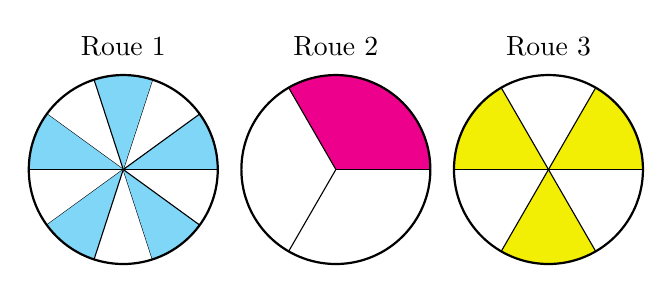
\begin{tikzpicture}[scale=0.6]
			% Roue 1
			\begin{scope}[xshift=-4.5cm]
				\node[above] at (0,2.2) {Roue 1};
				\foreach \i in {1,...,10} {
				\ifodd\i
					\fill[cyan!50] (0,0) -- ({(\i-1)*36}:2) arc ({(\i-1)*36}:{\i*36}:2) -- cycle;
				\fi
				\draw (0,0) -- ({\i*36}:2);
				}
				\draw[thick] (0,0) circle (2);
			\end{scope}

			% Roue 2
			\begin{scope}[xshift=0cm]
				\node[above] at (0,2.2) {Roue 2};
				\fill[magenta] (0,0) -- (0:2) arc (0:120:2) -- cycle;
				\draw (0,0) -- (0:2);
				\draw (0,0) -- (120:2);
				\draw (0,0) -- (240:2);
				\draw[thick] (0,0) circle (2);
			\end{scope}

			% Roue 3
			\begin{scope}[xshift=4.5cm]
				\node[above] at (0,2.2) {Roue 3};
				\foreach \i/\col in {1/yellow!80!lime, 3/yellow!80!lime, 5/yellow!80!lime} {
				\fill[\col] (0,0) -- ({(\i-1)*60}:2) arc ({(\i-1)*60}:{\i*60}:2) -- cycle;
				}
				\foreach \i in {1,...,6} {
						\draw (0,0) -- ({\i*60}:2);
					}
				\draw[thick] (0,0) circle (2);
			\end{scope}
		\end{tikzpicture}
	\end{center}
	Tous les secteurs angulaires d'une même roue ont la même mesure.

	Le joueur doit choisir une des trois roues et la lancer. Il remporte un lot s'il tombe sur un secteur coloré.

	Quelle roue le joueur doit-il choisir ?
\end{exo}
